\documentclass[sigconf,nonacm]{acmart}
\usepackage{tikz}
\usepackage{graphicx}
\usetikzlibrary{shapes.geometric, arrows.meta, positioning}

\AtBeginDocument{%
  \providecommand\BibTeX{{%
    \normalfont B\kern-0.5em{\scshape i\kern-0.25em b}\kern-0.8em\TeX}}}


\begin{document}

\title{Multi-Agent Debate System for News Credibility: Architecture and Usage Guide}

\author{Gideon Hale}

\maketitle

\section{System Architecture Overview}
The system takes in metadata about news articles and runs it through a structured multi-agent debate system, which ultimately returns a score on the reliability of the news article. 

\begin{figure}[h]
\centering
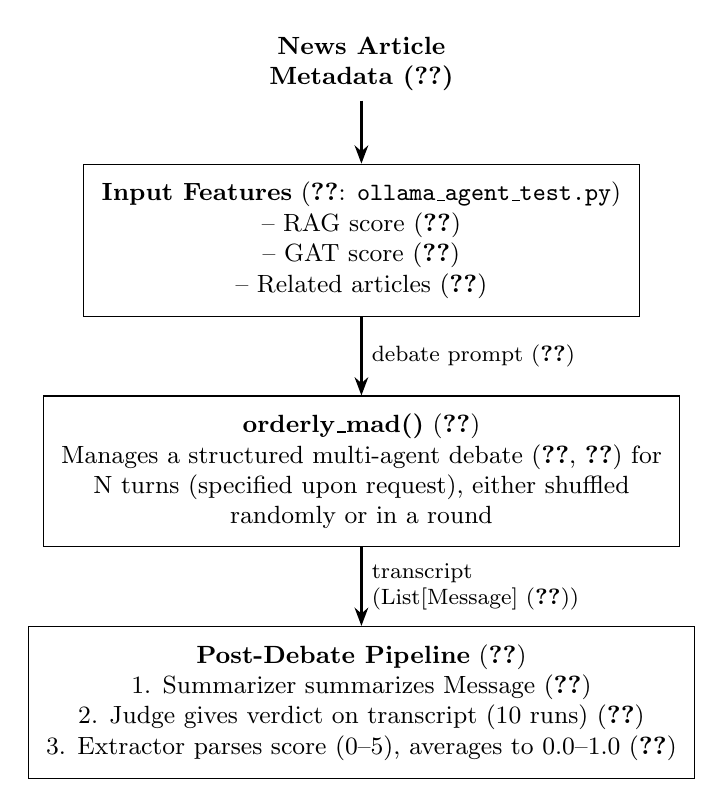
\begin{tikzpicture}[
  node distance=1.5cm,
  box/.style={draw, rectangle, align=center, minimum width=6cm, minimum height=1cm, inner sep=1.5ex, font=\small},
  arrow/.style={-{Stealth}, thick}
]

% Nodes
\node (json) [text width=4cm, align=center, font=\small\bfseries] {News Article Metadata (\ref{sec:input_data})};

\node (extractor) [box, below=0.8cm of json] {
    \textbf{Input Features} (\ref{sec:pipeline}: \texttt{ollama\_agent\_test.py}) \\
    -- RAG score (\ref{sec:input_data}) \\
    -- GAT score (\ref{sec:input_data}) \\
    -- Related articles (\ref{sec:input_data})
};

\node (mad) [box, below=1cm of extractor] {
    \textbf{orderly\_mad()} (\ref{sec:orderly_mad}) \\
    Manages a structured multi-agent debate (\ref{sec:agent_pool}, \ref{sec:roles}) for \\
    N turns (specified upon request), either shuffled \\
    randomly or in a round
};

\node (post) [box, below=1cm of mad] {
    \textbf{Post-Debate Pipeline} (\ref{sec:extraction}) \\
    1. Summarizer summarizes Message (\ref{sec:agent_pool}) \\
    2. Judge gives verdict on transcript (10 runs) (\ref{sec:agent_pool}) \\
    3. Extractor parses score (0--5), averages to 0.0--1.0 (\ref{sec:agent_pool})
};

% Arrows
\draw [arrow] (json) -- (extractor);
\draw [arrow] (extractor) -- node[right, align=left, font=\footnotesize] {debate prompt (\ref{sec:pipeline})} (mad);
\draw [arrow] (mad) -- node[right, align=left, font=\footnotesize] {transcript \\ (List[Message] (\ref{sec:core_agent}))} (post);

\end{tikzpicture}
\caption{System Event Timeline and Flow\label{fig:flow}}
\end{figure}

The workflow is summarized as follows:
\begin{enumerate}
    \item \textbf{Input Feature Extraction}: An input metadata file of a news article (in JSON format) is parsed to extract retrieval-augmented generation (RAG) signals, graph attention network (GAT) scores, and related articles.
    \item \textbf{Multi-Agent Debate}: The \texttt{orderly\_mad()} engine runs an $N$-turn debate among randomized agents reacting to the prompt.
    \item \textbf{Post-Debate Pipeline}: A \textit{Summarizer} synthesizes the debate transcript; a \textit{Judge} and \textit{Extractor} are iteratively run ten times to render verdict messages (scored 0--5) and parse the numerical score. These 10 scores are averaged and normalized to a range of 0.0--1.0.
\end{enumerate}

\section{Input Data Summary}\label{sec:input_data}

\textcolor{red}{[Note: Insert reference here to the section detailing the input metadata structure once written]}

A summary of all the major input fields that the system takes in and feeds to the MAD system are outlined in \textbf{Table \ref{tab:signals}}.

\begin{table}[h]
    \centering
    \caption{Summary of Input Processed Signals}
    \label{tab:signals}
    \resizebox{\columnwidth}{!}{%
    \begin{tabular}{llcl}
    \toprule
    \textbf{Signal} & \textbf{Source} & \textbf{Range} & \textbf{Purpose} \\
    \midrule
    Source Score & Adfontes & 0.0--1.0 & Avg. source reliability \\
    Missing Rate & RAG System & 0.0--1.0 & Coverage gap indicator \\
    Num Articles & RAG System & 0--30 & Corroboration volume \\
    Num Unrated & RAG System & 0--30 & Unknown-source volume \\
    GAT Score & Comment Graph & 0.0--1.0 & Topological credibility \\
    \bottomrule
    \end{tabular}%
    }
\end{table}

\section{System Components}\label{sec:components}

\subsection{Core Agent Abstraction (\texttt{ollama\_agent.py})}\label{sec:core_agent}
This module defines the foundational data types and agent behavior:
\begin{itemize}
    \item \textbf{\texttt{Message}}: A data class representing a single conversational turn with \texttt{role}, \texttt{content}, and \texttt{author}.
    \item \textbf{\texttt{Agent}}: A data class encapsulating a named persona with a system prompt, model identifier, temperature, and an OpenAI-compatible client. The \texttt{respond} method builds context and fetches the conversational LLM response.
\end{itemize}

\subsection{Instantiated Agent Pool (\texttt{agent\_presets.py})}\label{sec:agent_pool}
Configures and exports all named agents used in experiments, sharing an Ollama-backed endpoint. The primary agents mapped to the \textit{Journalist} persona and utility tools are outlined in \textbf{Table \ref{tab:roles}}.

\begin{table}[h]
    \centering
    \caption{Agent Roles and Configurations}
    \label{tab:roles}
    \begin{tabular}{lll}
        \toprule
        \textbf{Agent} & \textbf{Role} & \textbf{Model} \\
        \midrule
        Joseph & Journalist (investigative) & \texttt{mixtral:8x7b} \\
        Steven & Journalist (objective) & \texttt{gpt-oss:120b} \\
        Benjamin & Journalist (community) & \texttt{qwen2.5:72b} \\
        Christopher & Journalist (educational) & \texttt{mixtral:8x7b} \\
        Elijah & Journalist (misinfo specialist) & \texttt{gpt-oss:120b} \\
        Summarizer & Neutral observer & \texttt{qwen2.5:72b} \\
        Judge & Unbiased verdict-giver & \texttt{qwen2.5:72b} \\
        Extractor & Score extractor (0--5 format) & \texttt{mixtral:8x7b} \\
        \bottomrule
    \end{tabular}
\end{table}

It should be noted that the specific models assigned to these roles in \textbf{Table \ref{tab:roles}} are largely illustrative and somewhat arbitrary; the system architecture is model-agnostic and these debate and post-debate evaluation tasks could be executed just as effectively by any other capable, high-quality large language model.

\subsection{Role Definitions (\texttt{roles.py})}\label{sec:roles}
Provides a dictionary of system prompt templates keyed by specific domains such as journalist, mathematician, public administrator, and parent. Each role contains multiple persona variants providing ideological and methodological diversity within the debate. For the core evaluation of news articles, the system utilizes the "Journalist" domain, which defines five distinct personas. Each persona is assigned specific pedagogical instructions (task descriptions) that alter their approach to credibility assessment, as detailed in \textbf{Table \ref{tab:journalist_roles}}.

\begin{table}[h]
    \centering
    \caption{Journalist Personas and Task Descriptions}
    \label{tab:journalist_roles}
    \begin{tabular}{p{2cm} p{5.5cm}}
        \toprule
        \textbf{Persona} & \textbf{System Prompt / Task Description} \\
        \midrule
        Investigative & Focuses on holding the powerful accountable and exposing injustice through investigative reporting. \\
        Objective & Values objectivity and fairness, striving to present a balanced and impartial account of events. \\
        Community & Prioritizes community engagement and storytelling, amplifying the voices of ordinary people. \\
        Educational & Believes the media has a responsibility to educate the public and rigorously promote informed discourse. \\
        Misinformation Specialist & Excels specifically at identifying fake news, logical fallacies, and deliberate misinformation. \\
        \bottomrule
    \end{tabular}
\end{table}
\subsection{Debate Strategy and Orchestration (\texttt{orderly\_mad.py})}\label{sec:orderly_mad}
The \texttt{orderly\_mad()} engine is responsible for the synchronous execution of the multi-agent debate. It takes a discussion prompt, a list of agents, a maximum round count, and an agent ordering strategy. 

A critical vulnerability in multi-agent LLM systems is ``anchoring bias''—a phenomenon where the first agent to speak disproportionately influences the consensus trajectory of the ensuing debate. To mitigate this, \texttt{orderly\_mad()} implements dynamic strategies that allow for randomized permutation (`shuffle`) rather than strictly sequential execution (`round`). By shuffling the order of speakers per article, the system ensures that dissenting or highly critical personas (e.g., the Misinformation Specialist) have an equal probability of framing the initial argumentation. Over $N$ turns, this enforced adversarial structure prevents the formation of conversational echo chambers and forces the models to genuinely challenge conflicting viewpoints.

\subsection{Main Entry Point \& Pipeline (\texttt{ollama\_agent\_test.py})}\label{sec:pipeline}
Orchestrates the full credibility-assessment pipeline:
\begin{enumerate}
    \item Selects and loads an article metadata JSON file (from a selected pool in a subdirectory) by user request at the terminal.
    \item Extracts structured fields (RAG outputs, scores).
    \item Assembles a structured prompt describing debate rules, field descriptions, and article data.
    \item Executes the multi-agent debate.
    \item Runs the post-debate summarization, judgment, and extraction workflow iteratively, concluding in a final averaged reliability score from 0.0--1.0.
\end{enumerate}

\subsection{Evaluation and Deterministic Verdict Extraction}\label{sec:extraction}
Following the conclusion of the $N$-turn debate, the chaotic and lengthy transcript poses a challenge for direct scoring. LLMs tasked with simultaneous reasoning and strict numerical output formatting frequently fail at one of the two constraints. To resolve this, the architecture employs a tiered, three-agent post-debate pipeline:

\begin{enumerate}
    \item \textbf{Context Compression (Summarizer)}: A neutral observer agent processes the full debate transcript and generates a synthesized summary message. This prevents the downstream Judge from becoming distracted by conversational noise or overly dominating agents.
    \item \textbf{Decision Rendering (Judge)}: The \textit{Judge} agent receives the appended state array (`transcript + summary`). Relieved of the burden of exact formatting, it is instructed purely to synthesize the arguments and produce a qualitative explanation ending in a quantitative assessment (from 0--5).
    \item \textbf{Deterministic Parsing and Iteration (Extractor)}: Finally, an \textit{Extractor} agent operates solely on the Judge's verdict. Using a highly constrained system prompt, its only objective is to parse the Judge's rationale and predictably isolate the numerical value. To account for variance, the Judge and Extractor sequence is iterated ten times. The ten extracted scores (0--5) are then averaged and normalized to produce a robust final reliability score between 0.0 and 1.0.
\end{enumerate}
By conceptually separating reasoning (Judge) from formatting (Extractor), the system achieves a robust, deterministic programmatic output without sacrificing the nuanced ''Chain-of-Thought'' reasoning present in the debate.

\section{Architecture Justification}\label{sec:justification}
The multi-agent design of this framework intentionally decouples the subjective, nuanced reasoning of human-like debates from the strict structural constraints required for programmatic evaluation. By assigning diverse ideological personas to the active debaters, the system simulates a realistic unstructured "marketplace of ideas" where unverified claims are rigorously stress-tested. 

Furthermore, the post-debate pipeline introduces an elegant solution to two common computational limitations in conversational AI. First, LLMs empirically struggle with fine-grained numerical precision (such as judging accurately on a granular 0--100 scale), instead performing much more consistently and aligning closest to human intuition when working on a coarser 0--5 integer scale. Second, LLMs often fail to simultaneously perform deep reasoning while strictly adhering to rigorous output formatting. By restricting the Judge's primary evaluation to a 0--5 spectrum and employing a dual-agent mechanism—where the \textit{Judge} agent is granted complete freedom to construct unstructured ''Chain-of-Thought'' logic and the \textit{Extractor} agent simply parses the numerical intent—the architecture elegantly bypasses both issues. Iterating this final judgment phase ten times effectively smooths out the stochastic variance inherent to generative models, allowing the extracted evaluations to be reliably averaged and normalized into a robust, mathematically sound final score between 0.0 and 1.0.

\section{Experimental Results and Analysis}\label{sec:results}
To evaluate the effectiveness of our system, we conducted an experiment analyzing the multi-agent debate (MAD) reliability scoring against the Inference Dataset. After removing extreme outliers and extracting the intersecting test results, we successfully matched our output against actual ground-truth data. The outcomes of this evaluation are thus presented graphically.

\subsection{Multi-Agent System Performance}
The relationship between the final evaluated MAD scores (averaged across 3 iterations with 5 judge iterations each) and actual labels (where 0 indicates unreliable and 1 indicates reliable) for our test entries is shown in \textbf{Figure \ref{fig:mad_scores}}. We were originally planning to do 5 iterations with 10 judge iterations, but due to time and computational constraints, we reduced it to 3 iterations with 5 judge iterations each.

\begin{figure}[h]
    \centering
    \textcolor{red}{[Note: Actually include the average\_vs\_actual\_plot.png figure here]}
    \caption{Average Reliability Score from the Multi-Agent Debate framework vs. Actual Ground Truth Label.}
    \label{fig:mad_scores}
\end{figure}

\subsubsection*{Score Normalization and Safety Hedging}
Notably, the raw evaluations revealed that the system never recommended any article with more than 80\% (0.8) positive confidence. This is likely attributable to "safety hedging"—a phenomenon where strongly aligned LLMs systematically avoid assigning absolute credibility to claims without infallible external proof. To account for this artificial ceiling, we normalized the dataset by establishing 0.8 as the new maximum possible confidence (mathematically dividing raw scores by a factor of 0.8) and strategically filtering out significant outliers from the test set.

\subsubsection*{Asymmetric Classification Analysis}
Prior to normalization, the average raw score assigned to a fabricated (false) post was 0.4416, while a verified (true) post averaged 0.5624. Once the scores were normalized cleanly around the 0.8 bounds, these averages effectively settled at 0.552 for false posts and 0.703 for true posts, respectively.

These distributions reveal a significant asymmetry in the system's analytical capabilities, indicating that there are noticeably fewer false positives than false negatives. Simply put: the system is markedly better at confirming when an article is trustworthy than identifying when it is untrustworthy.

When the system encounters a fabricated or unreliable post, its adjusted average judgment (0.552) essentially mirrors random chance—it is almost as likely to categorize an unreliable post as reliable as it is to correctly flag it. However, when parsing an honestly sourced, trustworthy post, the system correctly identifies it with roughly 70\% confidence on average.

Overall, while the orchestrated software architecture succeeds at simulating a robust debate, the empirical results underscore a critical disparity. The internal NLP-driven semantic debate functions decently as a verification tool for true claims but severely struggles to reliably penalize disinformation. Pushing these autonomous systems to production will necessitate extensive calibration to correct this false-negative bias, potentially expanding them by integrating hybrid verification signals that retrieve external knowledge dynamically rather than relying solely on frozen metadata and semantic parsing.

\subsection{Methodological Limitations and Retrospective}
While the experimental pipeline mechanically functioned as intended, several critical design limitations likely hampered the system's absolute accuracy and statistical conclusiveness. Identifying exactly what could have been optimized or structured better during the experimentation phase provides vital context for interpreting the scatterplot:

\begin{itemize}
    \item \textbf{Sample Size and Class Imbalance}: The evaluation dataset consisted of merely 100 aligned ground-truth test results before outlier trimming. This dramatically constrained the statistical significance of the results. A substantially larger sample size (e.g., thousands of historical posts) could have revealed subtle macro-clustering trends that are currently completely drowned out by noise in the small-scale scatter plot.
    \item \textbf{Exclusively Open-Weight Models}: The \textit{Judge} and \textit{Extractor} agents were deliberately restricted to locally hosted, open-weight models (such as \texttt{qwen2.5:72b} and \texttt{mixtral:8x7b}) due to local constraints. Without establishing a robust control baseline utilizing frontier proprietary models (like GPT-4o or Claude 3.5 Sonnet), it remains incredibly difficult to isolate whether the poor classification separation was caused by systemic architectural failure or simply mid-tier reasoning ceilings.
    \item \textbf{Isolated Execution Environment}: The multi-agent debate was executed in a zero-shot, static vacuum fueled solely by the initial static JSON metadata. The experiment could have been vastly improved by equipping the debaters with real-time web-browsing capabilities or executable Python tools. Allowing the agents to query credible news databases directly rather than debating blindly over ambiguous RAG metrics would have likely grounded their arguments in objective reality.
    \item \textbf{Arbitrary Iteration Counts}: The Judge mechanism was prompted exactly 5 times to mathematically resolve variance. Retrospectively, for highly complex or polarized topics, 5 iterations might be functionally insufficient to overcome the initial random seed variance. A more rigorous, adaptive configuration utilizing dynamic stopping criteria (e.g., automatically iterating until the standard deviation of scores organically drops below a certain confidence threshold) would have yielded vastly more stable credibility evaluations.
    \item \textbf{Limited Computational Resources}: In running the experiment, it became clear, that the MAD system took up much more time and resources to execute than anticipated. This may be a hardware constraint that may be solved with more powerful computers or a more effective paralelization mechanizm, or some other optimization. Either way, it made running the experiment as originally intended impractical, which may have contributed to the lack of statistically significant results.
\end{itemize}

\section{Potential Future Work}\label{sec:future}
While the current architecture automates a form of credibility assessments via multi-agent debate, there are several promising avenues for future research and system enhancement:

\begin{itemize}
    \item \textbf{Real-Time Web Retrieval Tools}: Currently, the system relies on static metadata and pre-computed RAG features provided in the JSON input. Integrating live retrieval capabilities (e.g., web search APIs, direct database querying) would allow agents to actively fact-check emerging claims dynamically during the debate.
    \item \textbf{Hierarchical and Directed Debate Structures}: Exploring alternative orchestration strategies beyond flat shuffling or round-robin execution. Implementing structured hierarchical debate formats—where sub-agents debate specific claims and report back to a primary analytical agent—could improve the depth of the analysis.
    \item \textbf{Human-in-the-Loop Evaluation Baseline}: Conducting empirical evaluation of the system's accuracy and ideological balance by comparing its extracted credibility scores (0.0--1.0) against expert annotations from professional human fact-checking organizations such as PolitiFact or Reuters.
    \item \textbf{Expanded Persona Topologies}: Broadening the scope of the instantiated agent pool (\texttt{agent\_presets.py}) to include highly specialized domains (e.g., medical experts for health-related news, or legal analysts for policy news) can provide more nuanced scrutiny, specifically targeting domain-level misinformation.
\end{itemize}

\end{document}
